\documentclass{article}

\usepackage[a4paper, total={6in, 8in}]{geometry}

\usepackage{amsmath}
\usepackage{amsfonts}
\usepackage{amssymb}
\usepackage[T1, T2A]{fontenc}
\usepackage[utf8]{inputenc}
\usepackage[english, russian]{babel}
\usepackage{graphics}
\usepackage{graphicx}
\usepackage{makecell}

\geometry{
 a4paper,
 total={170mm,257mm},
 left=20mm,
 top=20mm,
 }

\author{Петров Артём Антонович, группа 721}
\title{Лабораторная работа № 3.3.4 "Эффект Холла в полупроводниках"}

\begin{document}
   
\begin{minipage}[t][4cm]{\textwidth}
\maketitle
\end{minipage}   
   
   \paragraph{Цель работы:} измерение подвижности и концентрации носителей заряда в полупроводниках.
   
   \paragraph{В работе используются:} электромагнит с источником питания, амперметр, миллиамперметр, милливеберметр, реостат, цифровой вольтметр, источник питания ($1.5$В), образцы легированного германия.
   
   \subsubsection*{Экспериментальная установка:}
   
   \begin{figure}[h]
   \centering
   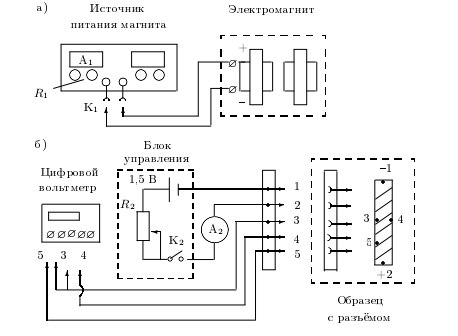
\includegraphics[width=15cm]{3_3_4.jpg} 
   \caption{Схема установки для исследования эффекта Холла в полупроводниках. $A_1, A_2$ - амперметры. Разъём $K_1$  позволяет менять направление тока в обмотках электромагнита. Реостат $R_2$ регулирует силу тока, текущего через образец при замыкании ключа $K_2$.}
   \label{fig.1} 
   \end{figure}

	Следует помнить, что контакты выводов 3 и 4 могут быть припаяны не идеально напротив друг друга. Для учитывания возникающий из-за этого ошибки измерения Холловской ЭДС следует замерить дополнительно возникающую разность потенциалов и вычитать её из показаний вольтметра при измерениях.
	
	Также следует откалибровать электромагнит (получить зависимость $B(I_1)$ для последующего задания индуктивности магнитного поля) с помощью милливеберметра перед началом измерений.

	Для вычисления проводимости образца можно воспользоваться следующей формулой: $$ \sigma = \frac{IL_{35}}{U_{35}al} $$ где a,l - ширина и толщина образца соответственно, $L_{35}$ и $U_{35}$ - расстояние и напряжение (в отсутствии магнитного поля) между контактами 3-5.
	 
	\newpage
   \subsection*{Обработка результатов}
   Построим график зависимости $B(I_{\text{м}})$, чтобы определять индукцию магнитного поля по току в катушке (рис. \ref{fig.2}).
   
   \begin{figure}[h]
   \centering
   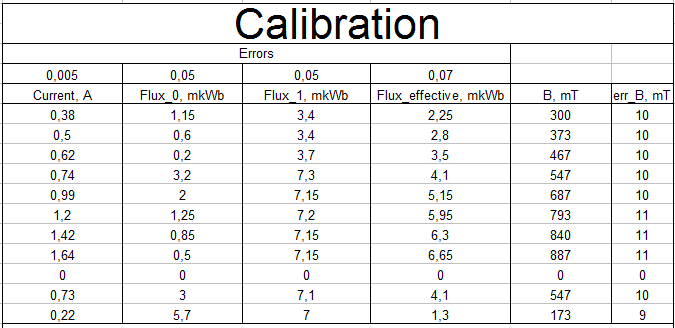
\includegraphics[width=15cm]{Table1.png} 
   \caption{Зависимость $B(I_{\text{м}})$} 
   \label{t1} 
   \end{figure}

   
   
   \begin{figure}[h]
   \centering
   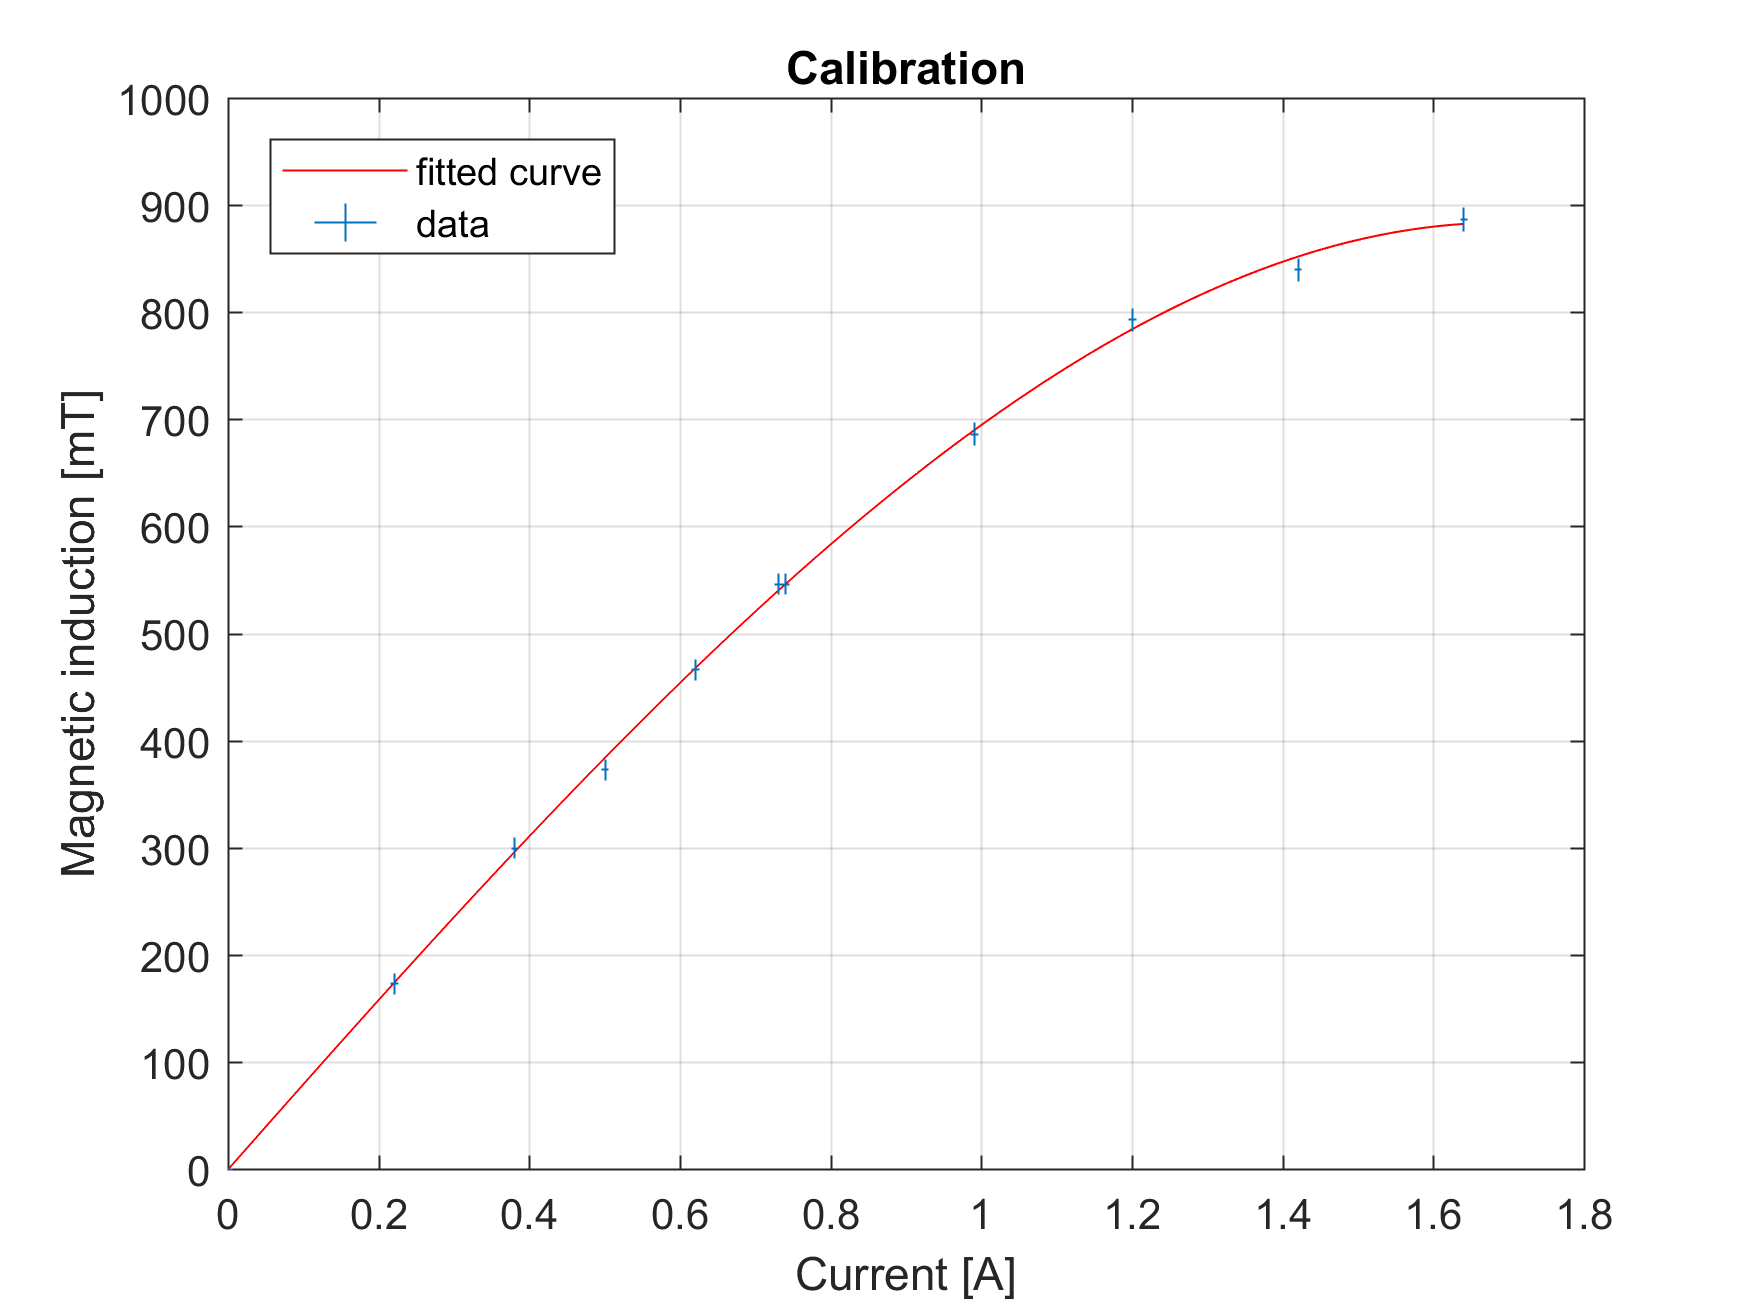
\includegraphics[width=12cm]{CalibrationPlot.png} 
   \caption{Зависимость $B(I_{\text{м}})$} 
   \label{fig.2} 
   \end{figure}

   Рассчитаем ЭДС Холла по формуле 
   $$ \varepsilon_{\text{х}} = U_{34} - U_0 $$
   и построим графики  $\varepsilon_{\text{х}}(B)$ для различных $I_0$ ( рис. \ref{fig.exb1}). Для каждого графика посчитаем коэффициент наклона $k(I_0) = \Delta\varepsilon / \Delta B$. Построим график $k = f(I_0)$ (рис. \ref{fig.exb3}). Коэффициент его наклона:
   $$ K = 1.004 \pm 0.008 \text{ В/(Тл$\cdot$А)} $$
   
   \begin{figure}[ht]
   \centering
   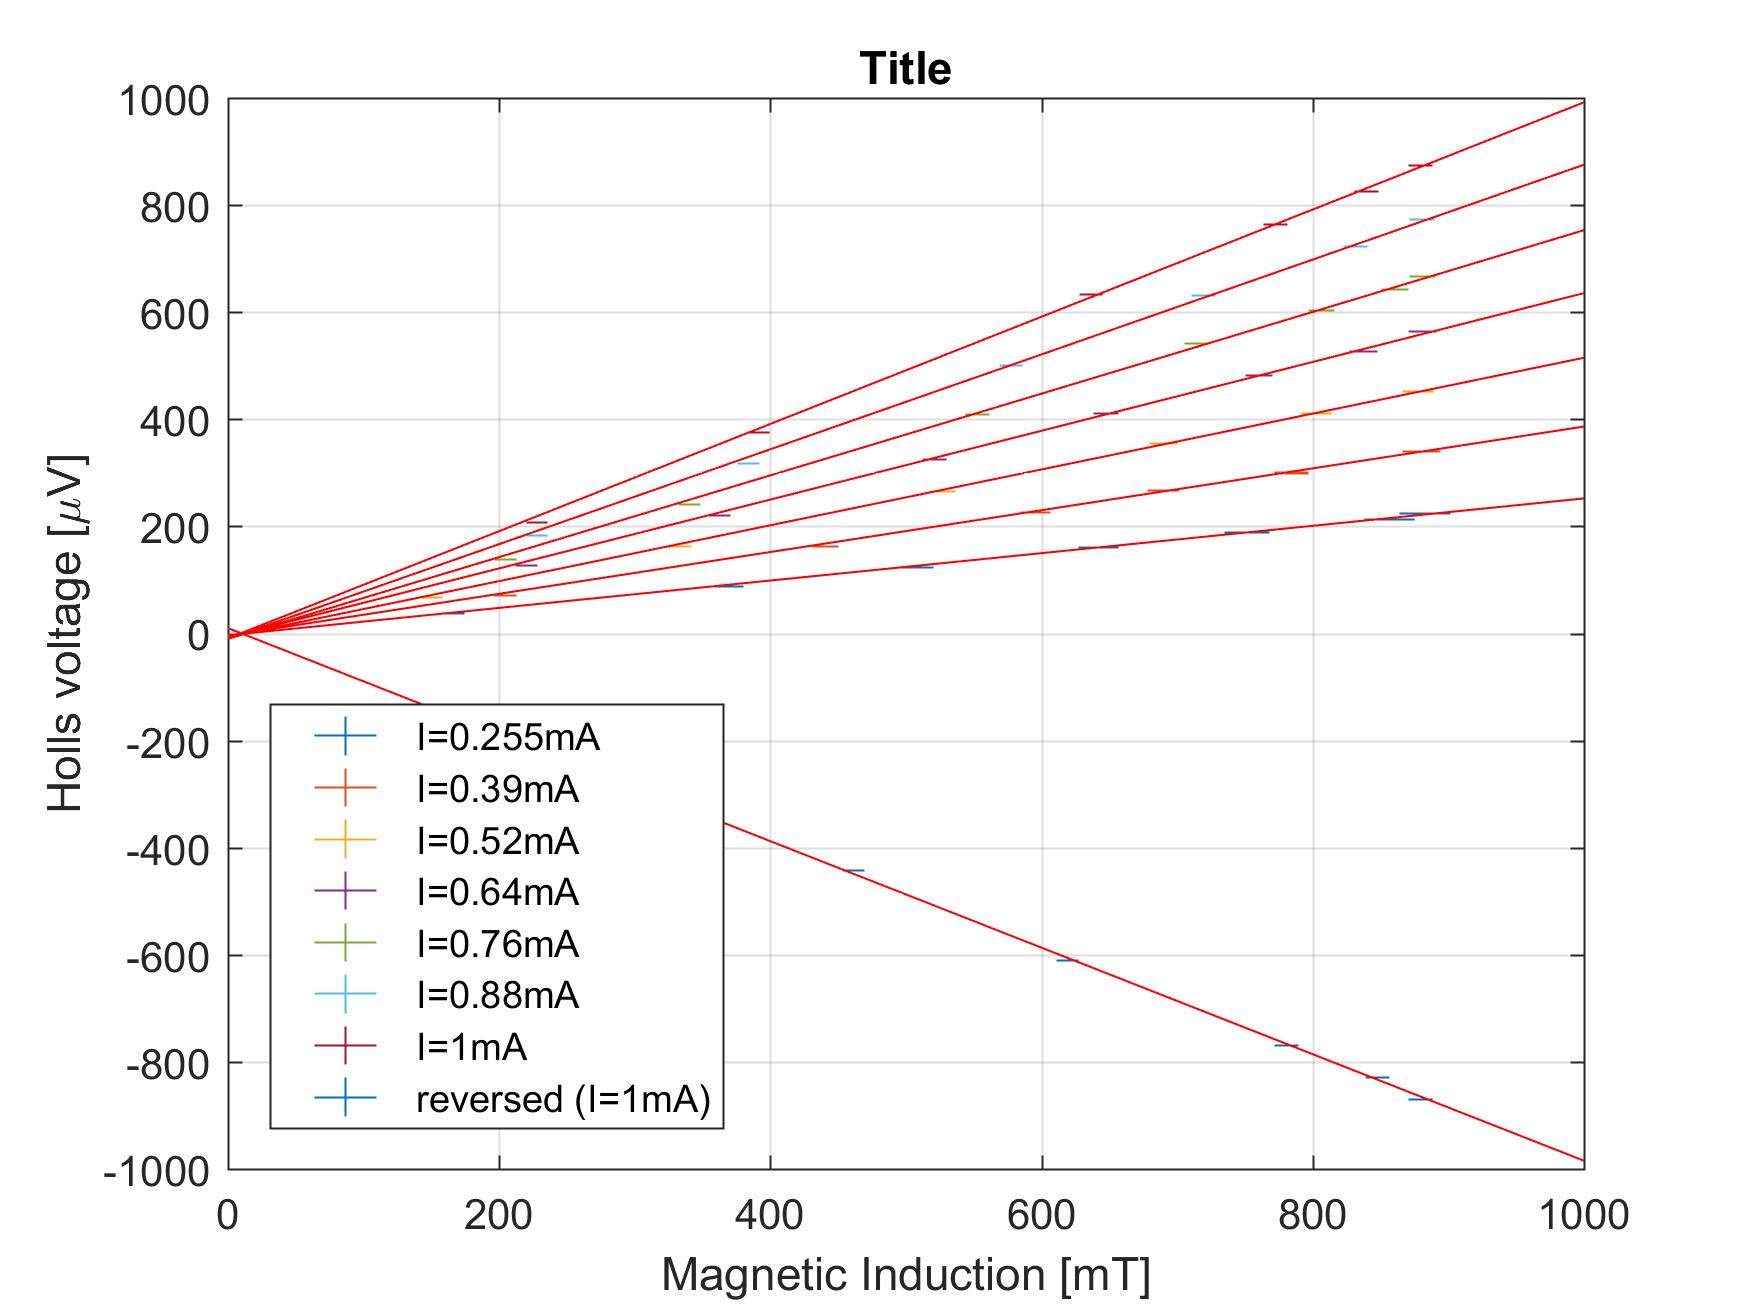
\includegraphics[width=12cm]{plot1.png} 
   \caption{Зависимость $\varepsilon_{\text{х}}(B)$ для различных $I_0$} 
   \label{fig.exb1} 
   \end{figure}

	\newpage 
	
	\begin{figure}[ht]
   \centering
   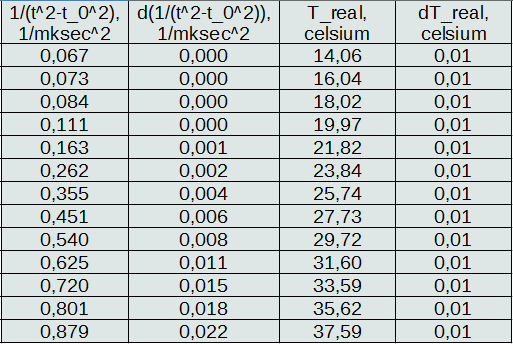
\includegraphics[width=7cm]{table2.png} 
   \caption{Зависимость $k(I_0) = \Delta\varepsilon / \Delta B$ для различных $I_0$} 
   \label{fig.exb2} 
   \end{figure}
   
   \begin{figure}[ht]
   \centering
   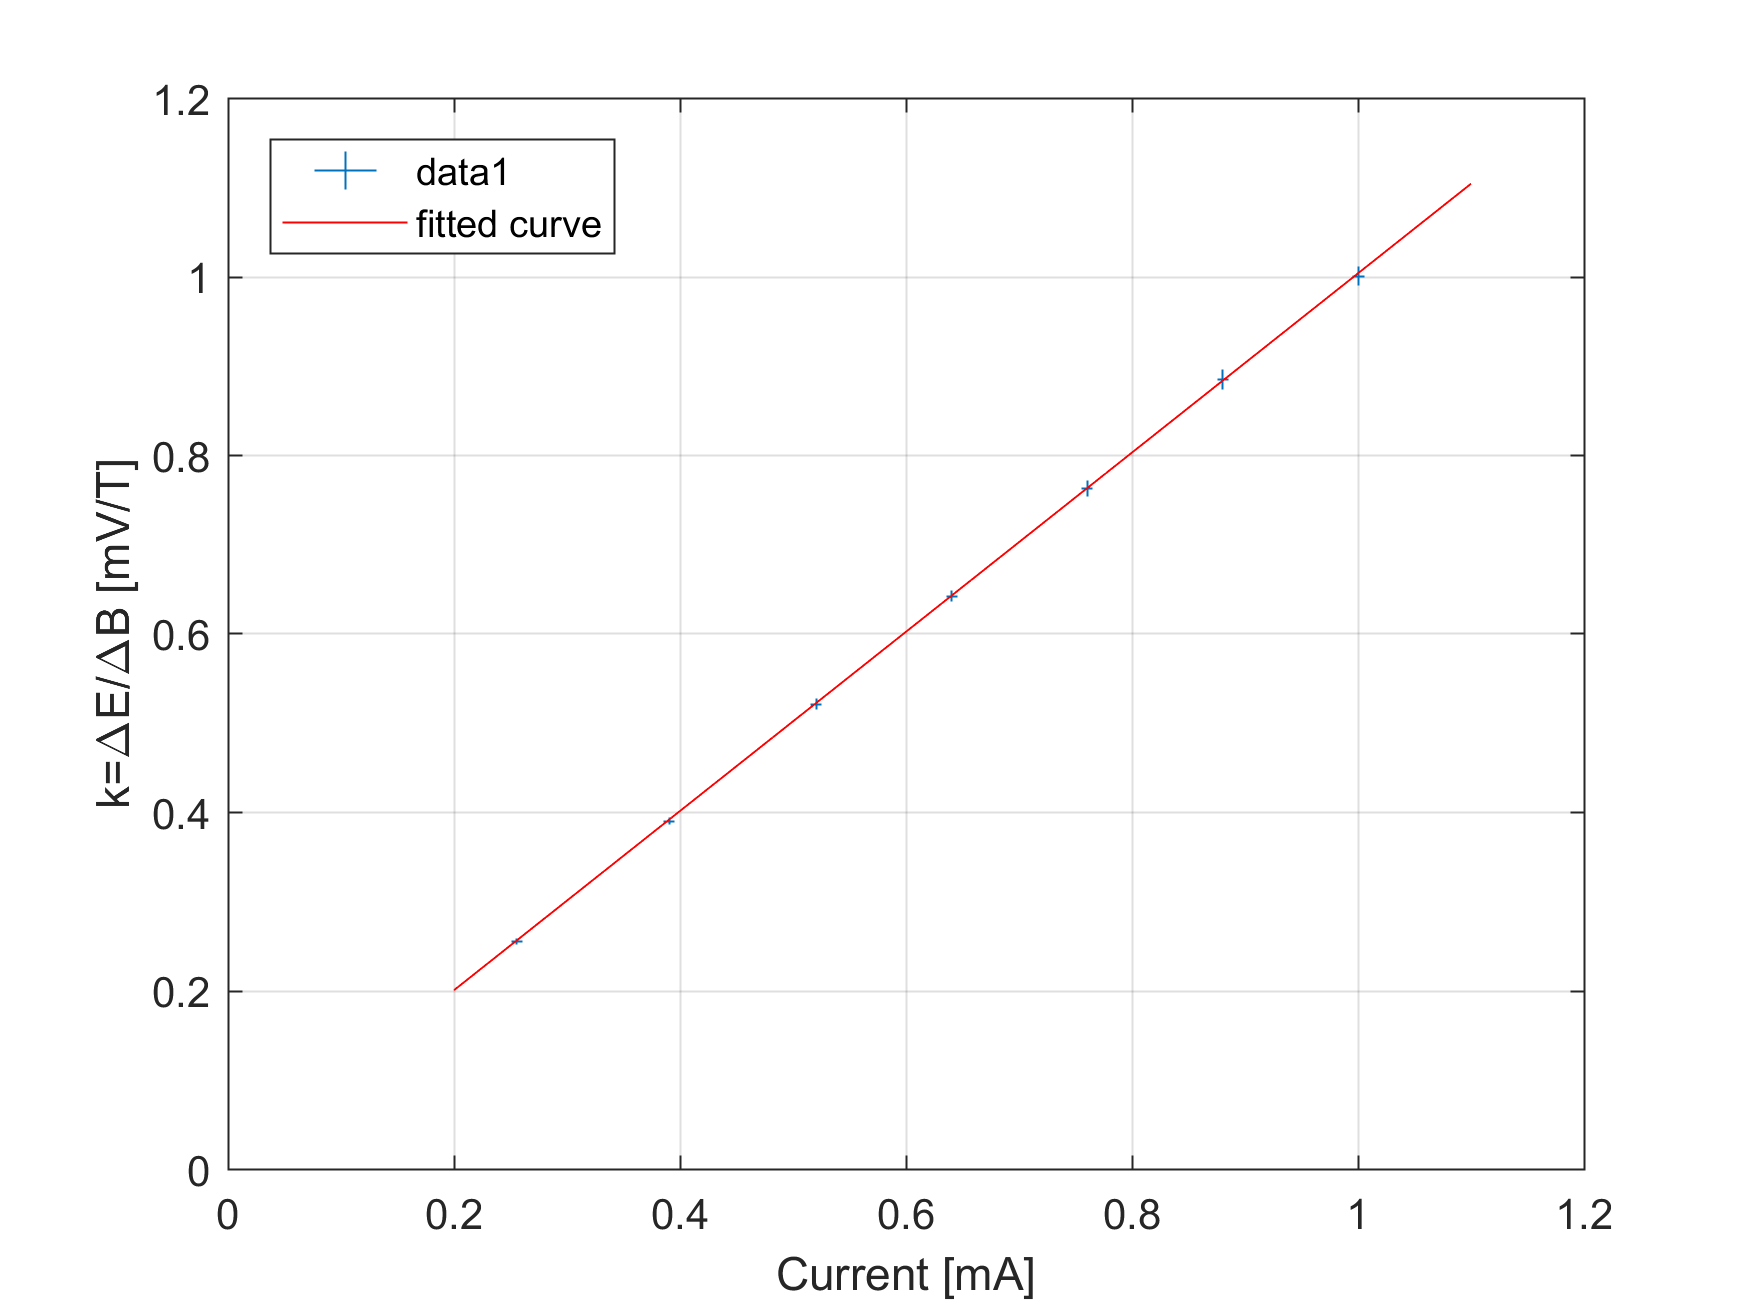
\includegraphics[width=15cm]{plot2.png} 
   \caption{Зависимость $k(I_0) = \Delta\varepsilon / \Delta B$ для различных $I_0$} 
   \label{fig.exb3} 
   \end{figure}
   
   Выражение для коэффициента Холла:
   $$ \varepsilon_{\text{х}} = -R_{\text{х}} \cdot \frac{I_0B}{a},~~ \frac{\varepsilon_{\text{х}}}{B} = -\frac{R_{\text{х}}}{a} I_0,~~ k = KI_0,~~ K = - \frac{R_\text{х}}{a}$$ 
   $$ R_{\text{х}} = -\frac{K}{a},~~ \sigma_{R_\text{х}} = \frac{K}{a^2}\sigma_a $$
   $$ R_\text{х} = (-1.00 \pm 0.06)*10^{-3} ~~\text{м}^3 / \text{Кл} $$
   
	Результат не совпадает с таблицей, где порядок $R_\text{х}$ равен 0.1 $\text{м}^3 / \text{Кл}$. С другой стороны, непонятно, какие примеси были использованы в данном образце и поэтому значение $R_\text{х}$ может отличаться от табличного для примесей Sb и Sb+Si.
   
   Концентрания носителей тока:
   $$ n = \frac{1}{R_xe} $$
   $$ n = (6.2 \pm 0.4) \cdot 10^{21} ~ \text{м}^{-3} $$
   
   Здесь аналогичное расхождение с таблицей ($\sim 10^{20}$).

~

   \noindentРассчитаем удельную проводимость $\sigma$ по формуле:
   $$ \sigma = \frac{IL_{35}}{U_{35}al}$$
   $$ \sigma = (1.29 \pm 0.10)~ (\text{Ом$\cdot$м})^{-1} $$
 
 	Результата совпадает с табличными данными по порядку величины ( 1 $(1/\text{Ом$\cdot$м})$).

   \noindentВычислим подвижность носителей тока:
   $$ b = \frac{\sigma}{en}$$
   $$ b = (12.4 \pm 1.3)~ \text{см}^2 / (\text{В} \cdot \text{с}) $$
   

   \paragraph*{Вывод.} В ходе данной работы были получены значения постоянной Холла, удельной проводимости и подвижности носителей тока для легированного германия. Сравнение с таблицей выдало совпадение только  в случае проводимости, что позволяет говорить о наличии некоторых нестандартных примесей. Также был определён тип проводимости (электронная).

\end{document}
